%%%%%%%%%%%%%%%%%%%%%%%%%%%%%%%%%%%%%%%%%
% baposter Landscape Poster
% LaTeX Template
% Version 1.0 (11/06/13)
%
% baposter Class Created by:
% Brian Amberg (baposter@brian-amberg.de)
%
% This template has been downloaded from:
% http://www.LaTeXTemplates.com
%
% License:
% CC BY-NC-SA 3.0 (http://creativecommons.org/licenses/by-nc-sa/3.0/)
%
%%%%%%%%%%%%%%%%%%%%%%%%%%%%%%%%%%%%%%%%%

%----------------------------------------------------------------------------------------
%	PACKAGES AND OTHER DOCUMENT CONFIGURATIONS
%----------------------------------------------------------------------------------------

\documentclass[landscape,a0paper,fontscale=0.285]{baposter} % Adjust the font scale/size here

\usepackage{graphicx} % Required for including images
\graphicspath{{figures/}} % Directory in which figures are stored

\usepackage{amsmath} % For typesetting math
\usepackage{amssymb} % Adds new symbols to be used in math mode

\usepackage{booktabs} % Top and bottom rules for tables
\usepackage{enumitem} % Used to reduce itemize/enumerate spacing
\usepackage{palatino} % Use the Palatino font
\usepackage[font=small,labelfont=bf]{caption} % Required for specifying captions to tables and figures

\usepackage{multicol} % Required for multiple columns
\usepackage{bigints}
\usepackage{url}
\setlength{\columnsep}{1.5em} % Slightly increase the space between columns
\setlength{\columnseprule}{0mm} % No horizontal rule between columns

\usepackage{tikz} % Required for flow chart
\usetikzlibrary{shapes,arrows} % Tikz libraries required for the flow chart in the template

\newcommand{\compresslist}{ % Define a command to reduce spacing within itemize/enumerate environments, this is used right after \begin{itemize} or \begin{enumerate}
\setlength{\itemsep}{1pt}
\setlength{\parskip}{0pt}
\setlength{\parsep}{0pt}
}

%\definecolor{lightblue}{rgb}{0.145,0.6666,1} % Defines the color used for content box headers
\definecolor{lightblue}{rgb}{1,0.3333,0.3333} %not very 'light blue'

\begin{document}

\begin{poster}
{
headerborder=closed, % Adds a border around the header of content boxes
colspacing=1em, % Column spacing
bgColorOne=white, % Background color for the gradient on the left side of the poster
bgColorTwo=white, % Background color for the gradient on the right side of the poster
borderColor=lightblue, % Border color
headerColorOne=black, % Background color for the header in the content boxes (left side)
headerColorTwo=lightblue, % Background color for the header in the content boxes (right side)
headerFontColor=white, % Text color for the header text in the content boxes
boxColorOne=white, % Background color of the content boxes
textborder=roundedleft, % Format of the border around content boxes, can be: none, bars, coils, triangles, rectangle, rounded, roundedsmall, roundedright or faded
eyecatcher=true, % Set to false for ignoring the left logo in the title and move the title left
headerheight=0.1\textheight, % Height of the header
headershape=roundedright, % Specify the rounded corner in the content box headers, can be: rectangle, small-rounded, roundedright, roundedleft or rounded
headerfont=\Large\bf\textsc, % Large, bold and sans serif font in the headers of content boxes
%textfont={\setlength{\parindent}{1.5em}}, % Uncomment for paragraph indentation
linewidth=2pt % Width of the border lines around content boxes
}
%----------------------------------------------------------------------------------------
%	TITLE SECTION 
%----------------------------------------------------------------------------------------
%
{
\includegraphics[height=4em]{IITlogo.png}} % First university/lab logo on the left
{\bf\huge{\hspace{-1.5in}The Advancement of Cooling \\ \hspace{-1.5in}Absorbers in COSY Infinity}\vspace{0.1em}} % Poster title
{{ \large{\hspace{-1.5in}J. Kunz, P. Snopok \hspace{12pt} Illinois Institute of Technology \\\hspace{-1.5in}M. Berz, K. Makino \hspace{12pt}Michigan State University \vspace{-0.4em}}}}
%{\textsc{ \large{J. Kunz, P. Snopok \hspace{12pt} Illinois Institute of Technology }}}
{
\includegraphics[height=6em]{MAPlogo.png}} % Second university/lab logo on the right

%----------------------------------------------------------------------------------------
%	Introduction
%----------------------------------------------------------------------------------------
\headerbox{Introduction}{name=introduction,column=0,row=0}{
\fontsize{0.13in}{1em}\selectfont{
Muons are useful for the study of \textbf{high energy phenomena}, since
\begin{itemize}
\item{they are fundamental (unlike protons), which means they offer clean
collisions and in a smaller facility, and}
\item{they to not emit synchrotron radiation (unlike electrons), and so
circular acceleration with a very compact footprint is possible.}
\end{itemize}
Muons are also useful as a \textbf{neutrino source}, since it is possible to make a source of neutrinos that is pure, intense, high energy, and both neutrinos and anti-neutrinos can be produced. This makes for a more precise measurement:
\begin{itemize}
\item{a pure beam means that we can understand the mixture of neutrinos in our beam very well,}
\item{an intense beam means that we can look for oscillation with lots of neutrinos,}
\item{a high energy beam means that the chance of seeing each neutrino is higher,}
\item{and the presence of neutrinos and anti-neutrinos means that we can measure the difference between matter and antimatter.}
\end{itemize}
Together these factors make for a very precise experiment. However, muons are not without their challenges:
% since their decay is into two neutrinos and one electron. 
%This is advantageous over other neutrino sources since the neutrino beam intensity will be proportional
%to the muon beam intensity. However, there are several challenges:
%\\
%
\begin{itemize}
\item{Muons are tertiary particles (protons $\rightarrow$ pions $\rightarrow$ muons), hence large initial phase space.}
\item{Muon mean rest frame lifetime is 2.2 $\mu$s.}
\item{\textbf{Ionization cooling} is the only technique fast enough to reduce the large initial beam size in a short enough time.}
\item{This requires the beam to traverse matter, where it loses momentum in all directions, with subsequent energy restoration in the longitudinal direction.}
\end{itemize}

The stochastic processes of interest are straggling (fluctuation
about a mean energy loss), angular scattering, and transverse
position corrections. All simulations were performed using an initial pencil beam of momentum 172 MeV/$c$ through 109 mm 
of liquid hydrogen. The step size for COSY was the full 109 mm. These data were also compared to two 
other codes, ICOOL \cite{icool} and G4Beamline \cite{g4bl}, where the step sizes were both 1 mm.
}
}

%----------------------------------------------------------------------------------------
%	COSY
%----------------------------------------------------------------------------------------

\headerbox{COSY Infinity}{name=cosy,column=1,span=2,row=0}{
\fontsize{0.13in}{1em}\selectfont{
\textbf{COSY Infinity} \cite{cosy} is an arbitrary-order beam dynamics simulation
and analysis code. It can determine high-order transfer
maps of combinations of particle optical elements of arbitrary
field configurations. However, stochastic effects (random effects, such
as those observed in cooling absorbers) do not fit well into the transfer map paradigm. For 
this reason, the development of stochastic processes in COSY is reported here.
\\

}
}

%----------------------------------------------------------------------------------------
%	RESULTS 1
%----------------------------------------------------------------------------------------

\headerbox{Results: Angular Scattering}{name=results,column=1,span=2,below=cosy}{
\fontsize{0.13in}{1em}\selectfont{
\begin{multicols*}{2}
\vspace{1em}
\begin{center}
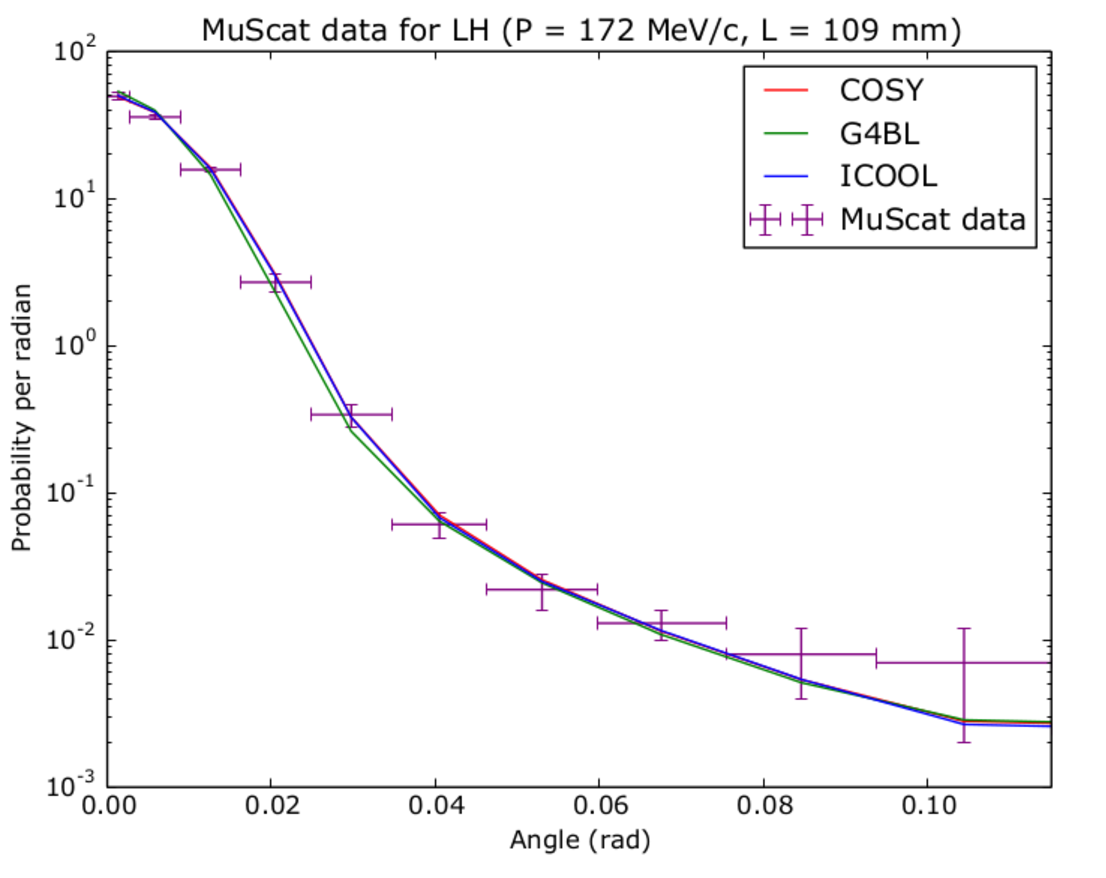
\includegraphics[width=\linewidth]{Figure2poster}
\captionof{figure}{Angular scattering comparison between COSY
(red), G4Beamline (green), ICOOL (blue), and the data
points from \cite{muscat} (purple).}
\end{center}
\columnbreak
\begin{itemize}
\item{Derivation for small and large angles performed separately.}
\item{Angular distribution peak is quite nearly Gaussian in $\theta$ \cite{gs}} up until some $u_0$.
\item{Tail follows the Mott cross section \cite{griffiths}.}
\item{Full distribution: 
\vspace{-0.3in}
\begin{center} \[g(u) = \left\{
  \begin{array}{lr}
    e^{-\frac{1}{2}\frac{1-u}{1-u_\sigma}} & |\text{ } u_0 < u\\
    \zeta\cdot\frac{1+\frac{1}{2}(\beta\gamma)^2(1+u-b)}{(1-u+b)^2} & | \text{ } u \le u_0
  \end{array} .
\right.
\] \end{center}}
\item{$u=$cos $\theta$.}
\item{$\zeta$, $b$ ensure continuity and smoothness.}
\item{$u_\sigma$, $u_0$ emperically chosen.}
\item{Good agreement is shown between COSY (red) and the MuScat experiment \cite{muscat} (purple).}
\end{itemize}
\end{multicols*}
}
}
%------------------------------------------------
\headerbox{Results: Transverse Phase Space}{name=posresults,column=1,span=2,row=1,below=results}{
\fontsize{0.13in}{1em}\selectfont{
\begin{multicols}{2}
\vspace{1em}
\begin{itemize}
\item{Transverse position depends on scattered angle $\theta$.}
\item{Picked out of Gaussian distribution with mean $\mu_T$ and standard deviation $\sigma_T$.}
\item{$\mu_T = \frac{\theta \rho_c L}{\mu_w}$.}
\item{ $\sigma_T = \max\Big(L \theta_\sigma \sqrt{\frac{1-\rho_c^2}{3}},\text{ }\Big|\frac{L P_T / P_Z}{\sigma_w}\Big|\Big).$}
\item{Model based on documentation by \cite{PDG}, with novel emperical parameters $\mu_w$ and $\sigma_w$.}
\item{Correlation coefficient: $\rho_c=\sqrt{3}/2$.}
\item{$\theta_\sigma$ corresponds to aforementioned $u_\sigma$.}
\item{$L$ is the absorber length; $P_T$, $P_Z$ are the (scattered) transverse and longitudinal momenta.}
\item{COSY phase space appears narrower. This may be misleading, as the discrepancy in not in the bulk but in the tails.}
\end{itemize}
\columnbreak
\begin{center}
\vspace*{0.1in}
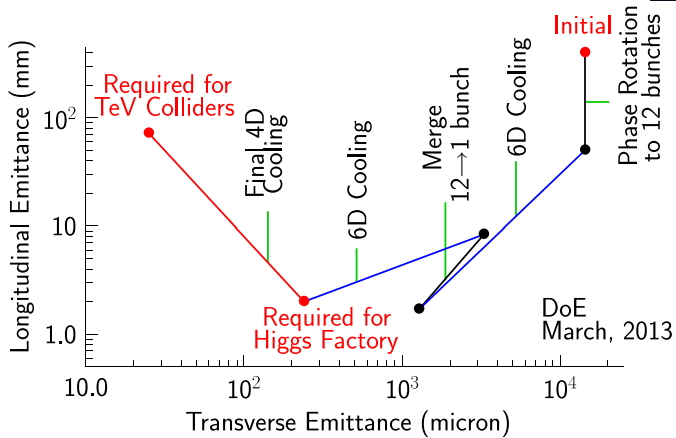
\includegraphics[width=\linewidth]{figure4}
\captionof{figure}{Transverse phase space comparison between COSY (red) and ICOOL (blue).}
\end{center}
\end{multicols}
}
}

%----------------------------------------------------------------------------------------
%	Eloss
%----------------------------------------------------------------------------------------

\headerbox{Results: Straggling}{name=eloss,column=3,row=0}{
\fontsize{0.13in}{1em}\selectfont{
\begin{center}
\includegraphics[width=\linewidth]{figure1poster}
\captionof{figure}{Straggling comparison between COSY (red), G4Beamline (green), and ICOOL (blue).}
\end{center}
\begin{itemize}
\item{Based on Landau theory \cite{landau}.}
%: \begin{center} $f(\lambda) = \frac{1}{\xi} \cdot \frac{1}{2\pi i} \bigintsss_{c+i \infty} ^{c-i \infty} \text{exp}(x\text{ ln } x + \lambda x) dx$.  \end{center}}
%\item{$\xi \propto Z\rho L/\beta^2 A$.}
%\item{$\lambda \propto dE/\xi - \beta^2 - \text{ln } \xi$.}
\item{Tail disagrees with G4Beamline. This could be due to a regard for both ionization and excitation cross sections (Landau theory only regards ionization) 
or the synthetic width correction algorithm that G4Beamline employs.}
\end{itemize}
}
}

%----------------------------------------------------------------------------------------
%	Conc
%----------------------------------------------------------------------------------------

\headerbox{Conclusions}{name=conc,column=3,below=eloss}{
\fontsize{0.13in}{1em}\selectfont{
\begin{itemize}
\item{Both transverse and longitudinal analyses agree well with ICOOL, G4Beamline, and experimental data (when available).}
\item{While not shown, it is reported here that good agreement hs been achieved between COSY and other data from \cite{muscat} (e.g. 3.73 mm of Be).}
\item{$\mu_T$ and $\sigma_T$ (transverse phase space parameters) may need further adjusting.}
\item{Further benchmarking should be done, but is expected to agree well.}

\end{itemize}
}
}

%----------------------------------------------------------------------------------------
%	REFERENCES
%----------------------------------------------------------------------------------------

\headerbox{References}{name=references,column=3,span=1,below=conc}{

\renewcommand{\section}[2]{\vskip 0.05em} % Get rid of the default "References" section title
%\nocite{*} % Insert publications even if they are not cited in the poster
%\fontsize{0.3cm}{1em}\selectfont{ % Reduce the font size in this block
\tiny{
\begin{thebibliography}{9}
\setlength\columnsep{15pt}
\begin{multicols}{2}
\bibitem{cosy}
M. Berz, K. Makino, COSY Infinity, \url{http://www.cosyinfinity.org} .
\vspace{-0.038in}
\bibitem{icool} 
R. C. Fernow \emph{et al.}, ICOOL Simulation Code, \url{http://www.cap.bnl.gov/ICOOL/} .
\vspace{-0.038in}
\bibitem{g4bl}
T. Roberts, G4beamline, \url{http://www.muonsinternal.com/muons3/G4beamline} .
\vspace{-0.038in}
\bibitem{gs}
S. Goudsmit and J. L. Saunderson (1940), Phys. Rev. 57, p. 24.
\columnbreak
\bibitem{griffiths}
D. Griffiths (2008) Introduction to Elementary Particles, 2nd Ed. 
\vspace{-0.038in}
\bibitem{muscat}
D. Attwood \emph{et al.} (2006), NIM B251, p. 41.
\vspace{-0.038in}
\bibitem{PDG}
J. Beringer \emph{et al.} (PDG) (2013) PR D86, 010001 chpt. 31.
\vspace{-0.038in}
\bibitem{landau}
L. Landau, J. Phys 8, p. 201.
\end{multicols}
\end{thebibliography}
}}

%----------------------------------------------------------------------------------------

\end{poster}

\end{document}